\documentclass[12pt,letterpaper,titlepage]{article}
\usepackage[latin1]{inputenc}
\usepackage{amsmath}
\usepackage{amsfonts}
\usepackage{amssymb}
\usepackage{tikz}
\usepackage{pgf}
\usetikzlibrary{arrows,automata}
\author{Dimitri Demergis \\ Jason Lee \\ Stephen Lombardi \\ Marcus McCurdy}
\title{CS544 Group 5 Protocol}
\begin{document}
\maketitle

\section{Introduction}
This paper defines a media streaming protocol that allows a properly implemented server application to stream media on demand to client applications.  
\section{Services}

\section{Messages}
Client-to-Server Messages
\begin{itemize}
\item \textbf{SessionRequestMessage} - This message is sent by the client to the server. It is used to notify the server that it should provision a new streaming session. It also includes the version numbers of the protocol the client supports.
\item \textbf{ChallengeResponseMessage} - This message is sent from the client to the server as part of the authentication process.  Upon receiving the ChallengeMessage, the client passes the received challenge value (as well as its own password) to a hash function and sends the result back to the server.
\end{itemize}
Server-to-Client Messages
\begin{itemize}
\item\textbf{SessionMessage} - This is the servers reply to the SessionRequestMessage. It tells the client what version of the protocol that will be used during the streaming session. It also contains the session id that will be used in further communication with the server.
\item \textbf{StreamMessage} - These messages are sent while the protocol is in the streaming state. They contain the actual data that is being streamed.
\item \textbf{ChallengeMessage} - This message is sent from the server to the client to begin the authentication process.  The message contains a challenge value to be generated by the server.  This message marks the transition from the Connecting state to the Authentication state. 	
\item \textbf{ChallengeResultMessage} - This message is sent from the server to the client to complete the authentication process.  Upon receiving the ChallengeResponseMessage, the server compares the result received from the client to its own result, and informs the client of success or failure.
\end{itemize}

\section{DFA}
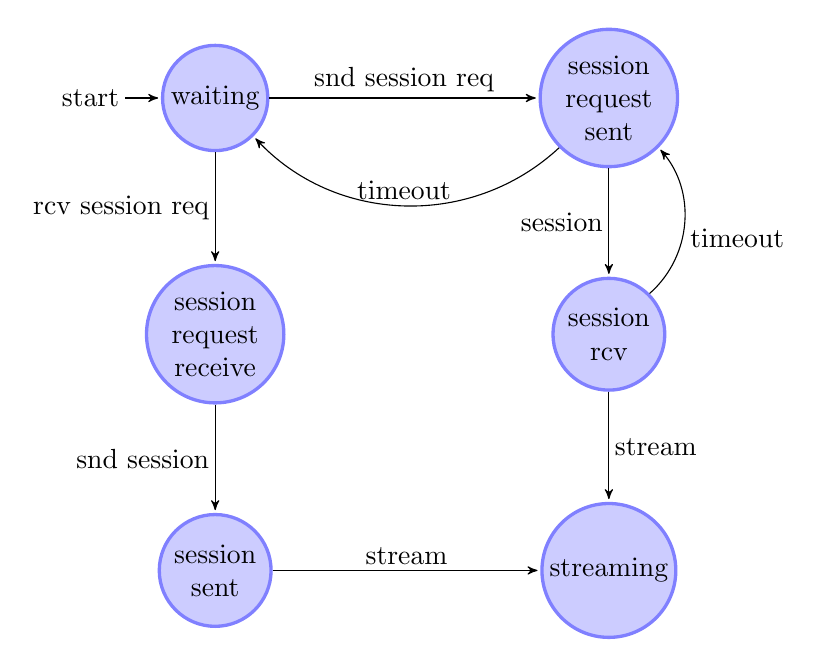
\begin{tikzpicture}[->,align=center,>=stealth',shorten >=1pt,auto,node distance=3cm,bend angle=45,inner sep=2pt, every state/.style={draw=blue!50,very thick,fill=blue!20}]
\node[initial,state] (waiting) {waiting};
\node[state, node distance=5cm] (session req sent) [right of=waiting] {session \\ request \\ sent};
\node[state] (session request receive) [below of=waiting]{session \\ request \\ receive};
\node[state] (ready) [below of=session request receive]{ready};
\node[state] (version sent) [below of=session request receive]{session \\ sent};
\node[state] (session receive) [below of=session req sent]{session \\ rcv};
\node[state] (streaming) [below of=session receive]{streaming};


\path (waiting) 		edge				node 			{snd session req} (session req sent)
	   					edge				node[swap] 		{rcv session req} (session request receive)
	(session req sent) 	edge [bend left]	node[swap] 		{timeout} 	(waiting)
						edge				node[swap]		{session} (session receive)
	(session request receive)		edge				node[swap]		{snd session}	(version sent)
	(session receive)		edge				node			{stream} (streaming)
						edge [bend right]	node[swap]		{timeout} (session req sent)
	(version sent)		edge				node			{stream} (streaming)
					
	;

\end{tikzpicture}

\section{Extensibility}
Protocol version information is included in connection messages so that the protocol version used by both sides can be established during the configuration phase.  This allows future improvements to the protocol to be implemented without rendering existing client applications unusable.

\section{Security}
This protocol uses a CHAP-like handshaking protocol for authentication of clients.  After the connection has been established, the server sends a challenge message to the client.  Both the client and server pass a password through a pre-determined hash function, and the server checks the results and informs the client of success or failure.
Since several different clients may be attempting to connect at the same time, the server must have a way to identify multiple simultaneous challenges that may be in various stages of the authentication process.

\end{document}